%%%%%%%%%%%%%%%%%%%%%%%%%%%%%%%%%%%%%%%%%%%%%%%%%%%%%%%%%%%
%
% Derived work from 
% https://www.overleaf.com/latex/templates/epfl-template-for-theses-and-projects/snkgdhbcrscn
%
% through modifications by Viktor Kuncak
%
% Goal: provide formatting for theses and project reports
%
%  
% the work from which it was derived had this notice:
%
% Author: Mathias Payer <mathias.payer@epfl.ch>
%
% This work may be distributed and/or modified under the
% conditions of the LaTeX Project Public License, either version 1.3
% of this license or (at your option) any later version.
% The latest version of this license is in
%   http://www.latex-project.org/lppl.txt
%%%%%%%%%%%%%%%%%%%%%%%%%%%%%%%%%%%%%%%%%%%%%%%%%%%%%%%%%%%
\documentclass[a4paper,11pt,oneside]{report}
% Options: MScThesis, BScThesis, MScProject, BScProject
\usepackage[MScThesis]{EPFLreport}
\usepackage{xspace}

\title{Java Mode for Simulating Native Image Behaviour}
\author{Ms Capucine Berger-Sigrist}

\newcommand{\sysname}{LogicCompiler\xspace}

\renewcommand{\committee}{ % shown on front page
\large
Thesis Advisor:\\
Viktor Kun\v{c}ak   % change if not in LARA
\\[1\baselineskip]

Company Advisor: \\ % for thesis in industry
Vojin Jovanovic \\[1\baselineskip] % change as needed, see next as well

PhD Student Supervisor: \\ 
Matthieu Bovel \\[1\baselineskip] % PhD student who helped in day to day supervision
} % end of committee command redefinition

\date{15 March 2024} % hand in date

\lstset{style=java_style}
\begin{document}
\maketitle
%\makededication
\makeacks

% We include individual parts using latex \include command: 
%    https://www.overleaf.com/learn/latex/Management_in_a_large_project

\begin{abstract}
% The abstract serves as an executive summary of your project.
% Your abstract should cover at least the following topics, 1-2 sentences for
% each: what area you are in, the problem you focus on, why existing work is
% insufficient, what the high-level intuition of your work is, maybe a neat
% design or implementation decision, and key results of your evaluation.

GraalVM Native Image compiles Java bytecode into a native image that operates under the closed-world assumption. This means that every reflectively-accessed element such as Class, Executable, or Field must be provided as reachability metadata to the image-build process. In Native Image, the reachability metadata is either 1) provided via user-provided configuration files in JSON format or 2) computed by partially evaluating the input program to pre-compute the reflectively-accessed elements.

Due to the long image-build times, creating the correct metadata is a time-consuming process for users: if the metadata for any element is missing, the entire image must be rebuilt. The objective of this project is to allow users to compute metadata with a quick turnaround by introducing a new mode to Java, so that it operates under the closed-world assumption and behaves exactly like Native Image.

We modify all reflective Java features to operate under the closed-world assumption by checking the reachability metadata to determine if the reflectively-accessed element is included in the image. We introduce a new Tracing Agent to collect the metadata. 
%% TODO check on the bytecode-to-bytecode partial evaluator move to future work
% To pre-compute the reflectively-accessed elements we implement a bytecode-to-bytecode partial evaluator that transforms classes before they are loaded and extracts reachability metadata from them. 
Finally, implementing the Java mode enables us to drive Native Image specifications and to clearly state what the expected behaviour is.   
\end{abstract}


\maketoc

\chapter{Introduction}

% The introduction is a longer writeup that gently eases the reader into your
% thesis~\cite{dinesh20oakland}. Use the first paragraph to discuss the setting.
% In the second paragraph you can introduce the main challenge that you see.
% The third paragraph lists why related work is insufficient.
% The fourth and fifth paragraphs discuss your approach and why it is needed.
% The sixth paragraph will introduce your thesis statement. Think how you can
% distill the essence of your thesis into a single sentence.
% The seventh paragraph will highlight some of your results
% Your core contribution should be in a subsection and use bullet points when possible. 
% You can refer to sections where the main results are shown. However, the purpose of contributions is 
% not to give an overview of the thesis text. Instead, the goal is to differentiate and crisply summarize the value of the thesis work. 
% You may optionally follow the contribution list with a plan of the thesis, if this adds something over the table of content. 
% This section is usually 3-5 pages.
%Therefore, no new element can be introduced at runtime.

GraalVM Native Image~\cite{noauthor_native_nodate} compiles Java bytecode into a standalone binary. It performs reachability analysis to compute a fixed set of classes from which it produces a binary. 
%This process assumes that all elements the application will need at runtime are known at \emph{build time}. This assumption is known as the \emph{closed-world assumption}.
This fixed set of reachable elements is known as the \emph{closed-world assumption}. Under this assumption, all the application's classes must be known at \emph{build time} to be included into the image.
However, dynamic features in Java, like reflection, can be used to access and load new classes at runtime, which contradicts the closed-world assumption. 

To overcome the limitations of the closed-world assumption and support Java's dynamic features, Native Image requires reflectively-accessed elements, that is, Classes, \emph{Executables} (i.e., Methods and Constructors), and Fields, to be specified in the \emph{reachability metadata}~\cite{noauthor_reachability_nodate}. The reachability metadata is passed to the image-build process and indicates which elements are reachable at runtime, and, thus, which elements must be included into the image. This metadata is either provided as a JSON configuration file or can be, in specific cases, pre-computed from user code. Concretely, invoking the method \verb|Class#forName(String)| of the Java Reflection API~\cite{noauthor_core_nodate} for a class \verb|C| requires to manually specify the entry \verb|{"name":"C"}| in the JSON configuration file.
To help collect the metadata, GraalVM provides a \emph{Tracing Agent}~\cite{noauthor_collect_nodate}. When running an application on a Java Virtual Machine~(JVM), the agent can be attached to the JVM to record the reflectively-accessed elements during an execution run and outputs a JSON configuration to pass to the image-build process.

Computing the reachability metadata is a tedious process. It requires the user to record in a JSON configuration each element of their application that might be introduced at runtime. While the Tracing Agent can provide the bulk of the metadata, it can still miss an element because the JVM does not behave the same way as Native Image. The agent may also have to be run multiple times to account for all the different execution paths. The Oracle GraalVM Reachability Metadata repository~\cite{noauthor_oraclegraalvm-reachability-metadata_2024} is another way to acquire the metadata for well-known open-source libraries but it also requires to be manually kept up to date.

At build time, Native Image performs analysis, applies multiple optimization phases, and compiles all the methods: creating an image takes time. In addition, if a single element is missing from the reachability metadata, the image crashes at runtime and must be rebuilt from the ground up. 

Unlike Java, Native Image does not have any specification for its semantics, and compiler optimizations can change the semantics of the program, this fact makes debugging the image a hazardous task.
Due to the issues with metadata collection, the long image build time and the lack of specifications, computing the correct reachability metadata is an altogether time-consuming process. 

By introducing a new mode to Java that simulates the semantics of Native Image, we can use Java to quickly test the reachability metadata without the overhead of building a new image each time. We refer to Java behaving according to Native Image's semantics as Java under native restrictions. To simulate the closed-world assumption, Java under native restrictions checks if each reflectively-accessed element is included in the reachability metadata. We address the issues with GraalVM's Tracing Agent by implementing a new Tracing Agent in Java that follows the same execution path as Java under native restrictions.

Because Native Image's semantics are not defined, we must first understand and define Native Image's behaviour before we attempt to simulate it in Java under native restrictions. Moreover, guaranteeing correctness requires rigorous testing when operating changes on a language runtime as widely used as Java. We run the Java Compatibility Kit~(JCK), a test suite with more than 100'000 tests, to verify that Java under native restrictions is as compliant with the Java Language Specification~\cite{noauthor_java_nodate-2} as Native Image is.
The last requirement is to keep changes to Java itself to a minimum. A line of code is introduced in the JDK only if removing it would break the correctness of the design.

Related projects attempt to bridge the gap between static and dynamic compilation for Java by combining both approaches. The aim is to optimize startup performance and resource utilization with AOT compilation while adding support for Java runtime features with just-in-time~(JIT) compilation. The premises of this thesis are different. We are already in a fully dynamic environment and are attempting to restrict Java's dynamic features to behave as if under a closed-world assumption, essentially tackling the problem the other way around. 

This thesis fits in an overall Native Image usability improvement plan. Porting Java to native restrictions allows users to compute metadata with a quick turnaround. It also enables us to both understand and validate the semantics of Native Image through execution. In turn, having a clear semantics drives the development of Native Image and makes debugging easier, as it leaves no room for unexpected behaviour.
The way we approached the implementation of Java under native restrictions is a cross between what could be coined "software archaeology", and "software surgery": we dug into the deepest parts of Java to understand how native restrictions could be applied to specific pieces of the code.

The main contributions of this thesis are the following:
\begin{itemize}
  \item We implement Java under native restrictions to simulate Native Image's behaviour for dynamic class loading, dynamic invocations and reflection
  \item With this implementation we drive Native Image's semantics, and provide the specification both in written form and with a Technology Compatibility Kit~(TCK) 
  \item We implement a new Tracing Agent in Java that follows Native Image's semantics to collect the metadata 
  \item We improve user's workflow by streamlining the computation of reachability metadata
\end{itemize}
%%%%%%%%%%%%%%%%%%%%%%%%%%%%%%
\chapter{Background}
%%%%%%%%%%%%%%%%%%%%%%%%%%%%%%

% The background section introduces the necessary background to understand your
% work. This is not necessarily related work but technologies and dependencies
% that must be resolved to understand your design and implementation.
% This section is usually 3-5 pages.

%%%%%%%%%%%%%%%%%%%%%%%%%%%%%%
\section{The Java Virtual Machine}
%%%%%%%%%%%%%%%%%%%%%%%%%%%%%%
Following the "write once, run anywhere" adage, the typical way of running a Java application is on a JVM.
The JVM offers an additional, target-independent, layer of abstraction between implementations of the Java programming language and the operating system itself.
The JVM is responsible for interpreting and executing Java bytecode, and provides four key components~\cite{dannarapu_jvm_2023-1}: 
the class loader to load classes into memory, the runtime data area (that is, the method area, heap, and stack) to store program data, the execution engine, which reads and executes bytecode instructions, and the garbage collector. The JVM Specifications~\cite{noauthor_java_nodate-1} describe in detail the requirements for a JVM to be compliant. 
The thesis targets a particular implementation, mainly Oracle's Java HotSpot~\cite{noauthor_hotspot_nodate} and its JIT compiler for Java 21. 
HotSpot relies on tiered compilation to optimize code execution. It consists of an interpreter and two JIT compilers: C1 and C2. 
C1 compiles bytecode with a minimal time and space overhead, applying only a limited set of optimizations, while C2 employs a more aggressive optimization strategy, requiring more resources.
The VM starts by interpreting the bytecode to minimize startup time, and collects profiling information at the same time. Using this information, once a method is deemed "hot" enough, C1 kicks in and starts compiling it. When the number of times the methods has been invoked (or the number of back-edges to that method) crosses another threshold, C2 recompiles the same code into a more optimized form. If an optimization is proven wrong, the code is deoptimized and the compiler reverts back to interpretations.  

%%%%%%%%%%%%%%%%%%%%%%%%%%%%%%
\section{GraalVM}
%%%%%%%%%%%%%%%%%%%%%%%%%%%%%%
GraalVM is a runtime ecosystem developed by Oracle Labs, and features three core components: the Graal compiler, Truffle~\cite{noauthor_truffle_nodate}, and Native Image.
Graal is a compiler that relies on multiple optimizations phases to produce optimized machine code from bytecode. The compiler operates on a language-agnostic intermediate representation called Graal~IR~\cite{duboscq_graal_2013}. Graal~IR not only facilitates the implementation of speculative optimizations, it also enables Graal to run guest programming languages (e.g., JavaScript, Python, Ruby) on the same JVM. 
The JVMCI~\cite{noauthor_jep_nodate}~(JVM Compiler Interface) API offers mechanisms to access the JVM internal data structures and install compiled code. Through this interface, Graal can integrate as a JIT compiler into HotSpot's system and replace C2. 
Graal can also be integrated with Native Image as the AOT compiler.

Native Image~\cite{wimmer_initialize_2019} is a compilation technology that compiles Java bytecode ahead-of-time into standalone binaries. This approach aims at reducing the startup time and memory footprint of Java applications. Native Image operates under the closed-world assumption, all Java classes, which includes the JDK, must be known at build time to be included in the image.
This also means, that every reflectively-accessed elements must be specified in reachability metadata to be made available to the build process. 
At build time, during static analysis, points-to-analysis and heap snapshotting are iteratively applied so that only reachable code remains in the final image. Additionally, part of the initialization code of the application can be executed at build time rather than at runtime.

%%%%%%%%%%%%%%%%%%%%%%%%%%%%%%
\section{Java's Dynamic Features}
%%%%%%%%%%%%%%%%%%%%%%%%%%%%%%
One of the cornerstones of the Java platform is its dynamic features. At run time, JARs, resources, and proxies can be loaded, and methods can be invoked without the compiler having seen them before. In the following section, we will dive deeper into the mechanisms of dynamic class loading and invocation.

%%%%%%%%%%%%%%%%%%%%%%%%%%%%%%
\subsection{Dynamic Class Loading}
%%%%%%%%%%%%%%%%%%%%%%%%%%%%%%
Dynamic class loading~\cite{liang_dynamic_1998} allows Java applications to load, link, and initialize classes at runtime. Plugins, for example, can be loaded and unloaded without restarting the application; dependency injection relies on late binding of dependencies, which is made possible with dynamic class loading. 

Class loaders are the underlying mechanism used for loading classes. 
There are two types of class loaders: the bootstrap (or system) class loader, which loads all the system classes, and user-defined class loaders, which load classes from user-defined sources.
Class loaders operate on a delegation model. If a class loader L directly loads C, then L is the \emph{defining loader} of C, otherwise L recursively delegate the loading to another class loader, until the defining loader of C is found. L is an \emph{initiating loader} of C. 
Concretely, a class loader in an instance of a subclass of the class \verb|ClassLoader|. 
Figure~\ref{fig:classloader}, shows the key methods of the class.

\begin{figure}[ht]
    \centering
\begin{lstlisting}[language=Java]
class ClassLoader {
    public Class<?> loadClass(String name);
    protected final Class<?> findLoadedClass(String name);
    static native Class<?> defineClass1(ClassLoader loader, String name, 
                                        byte[] b, int off, int len,
                                        ProtectionDomain pd, String source);
    static native Class<?> defineClass2(ClassLoader loader, String name, 
                                        java.nio.ByteBuffer b,
                                        int off, int len, ProtectionDomain pd,
                                        String source);
    static native Class<?> defineClass0(ClassLoader loader,
                                        Class<?> lookup,
                                        String name,
                                        byte[] b, int off, int len,
                                        ProtectionDomain pd,
                                        boolean initialize,
                                        int flags,
                                        Object classData);
    public static ClassLoader getSystemClassLoader();
    ...
}
\end{lstlisting}
    \caption{Core methods of the \texttt{ClassLoader} class}
    \label{fig:classloader}
\end{figure}


The method \verb|loadClass| is the usual entry point to initiate class loading. It can be called directly from user code, or triggered by a JVM instruction.
When loading a class \verb|C| with the system class loader (see Figure~\ref{fig:class_C}), the JVM first checks with the method \verb|findLoadedClass|, if \verb|C| has already been loaded, in which case it immediately returns the class, otherwise, the class loader attempts to locate the corresponding data. 

Linking a class or interface C is done in three steps: (1) the JVM verifies that the binary representation of the class or interface C is correct, (2) the static fields of C are created and initialized, and (3) symbolic references are resolved into direct references. If C has a direct superclass or superinterface D, then D must also be verified and prepared. 
Once all symbolic references have been resolved, the JVM invokes the method \verb|defineClass0|, \verb|defineClass1| or \verb|defineClass2| to transform the array of bytes into a run-time representation of the class, and returns a \verb|Class| object.

\begin{figure}[ht]
    \centering
\begin{lstlisting}[language=Java]
class C extends D {
}
class Main {
    public static void main(String[] args) {
        ClassLoader cl = ClassLoader.getSystemClassLoader();
        Class<?> c = cl.loadClass("C");
    }
}
\end{lstlisting}
    \caption{Dynamically loading the class C.}
    \label{fig:class_C}
\end{figure}

% \subsubsection{Native Image implementation}
% There are three main cases for how Native Image supports dynamic class loading: (1) the argument passed to \verb|loadClass| is a constant or is effectively constant, the argument is constant folded during static analysis, and gets compiled in the image, (2) the class is included in the reachability metadata, (3) the class is not a constant, nor is it registered, in which case the image will throw an exception at runtime.


% Every Java class used at build time is said to be build-time initialized. Note that merely loading a class does not necessarily initialize it. The static class initializer of build-time initialized classes executes on the JVM running the image build. If a class is initialized at build time, its static fields are saved in the produced binary. At run time, using such a class for the first time does not trigger class initialization.
% 
% Static analysis is a process that determines which program elements (classes, methods and fields) are used by an application. These elements are also referred to as reachable code. The analysis itself has two parts:

% Scanning the bytecodes of a method to determine what other elements are reachable from it.
% Scanning the root objects in the native image heap (i.e., static fields) to determine which classes are reachable from them. It starts from the entry points of the application (i.e., the main method). The newly discovered elements are iteratively scanned until further scanning yields no additional changes in element’s reachability.


%%%%%%%%%%%%%%%%%%%%%%%%%%%%%%
\subsection{The \texttt{invokedynamic} Instruction}
%%%%%%%%%%%%%%%%%%%%%%%%%%%%%%
The \verb|invokedynamic| instruction~\cite{noauthor_java_nodate} was introduced to support the invocation of methods without static type information at runtime.
This instruction is distinct from the JVM's traditional method invocation instructions (\verb|invokevirtual|, \verb|invokeinterface|, \verb|invokestatic|, and \verb|invokespecial|) in that it does not bind to a method at compile time. Instead, it defers the decision of which method to invoke until runtime.

At the core of the \verb|invokedynamic|'s resolution mechanism is the bootstrap method. A bootstrap method is a user-defined method that the JVM invokes the first time an \verb|invokedynamic| instruction is executed. Some bootstrap methods are provided by the JVM itself. For example, lambda expressions in Java use the \verb|LambdaMetafactory#metafactory| or \verb|altmetafactory| as their bootstrap methods. 
% Similarly, for performance reasons, the JVM now uses the \verb|invokedynamic| instruction for string concatenation~\cite{noauthor_jep_nodate-1}, the \verb|StringConcatFactory#makeConcat| is the bootstrap method.
This bootstrap method returns a \verb|CallSite| object, which encapsulates a target \verb|MethodHandle|. The \verb|MethodHandle| is a reference to an executable or a field and contains all the necessary mechanisms and data structure to invoke or access the object it references (e.g., the element's defining class, name, type signature, and methods to access it). 

\verb|CallSite| resolution involves three steps: (1) the bootstrap method handle is resolved, meaning all symbolic references to classes, interfaces, fields, and methods, as well as, all classes and interfaces contained in the method descriptor must be resolved, (2) the bootstrap method is invoked, and finally (3) the \verb|CallSite| is verified.
Once resolved, the \verb|CallSite| is cached and associated to a particular \verb|invokedynamic| instruction.
For subsequent invocations, the bootstrap method is not re-executed, instead the method handle encapsulated in the \verb|CallSite| can be directly invoked.

% The main difference between HotSpot's implementation of \verb|invokedynamic| and Native Image's resides in the \verb|CallSite| resolution. Native Image distinguishes how it handles \verb|CallSite| resolution based on whether the bootstrap method is JVM-implemented or not. For trusted, JVM-implemented bootstrap methods, resolution occurs at build time. Otherwise, the bootstrap method is interpreted at runtime and the resolution relies on reflection, requiring the declaring class, the method and the method types to be registered for reflection.

% This MethodHandle effectively directs subsequent invocations of the invokedynamic instruction, bypassing the need for further resolution. The ability to specify the bootstrap method, along with the CallSite and MethodHandle it produces, allows for dynamic language behaviors such as runtime method linking and method invocation based on runtime conditions rather than static analysis.

%    Any exception that can be thrown as a result of failure of resolution of a symbolic reference to a method type can be thrown in this step.


% Each invokedynamic has a known bootstrap method given as its compile-time parameter. Whenever a invokedynamic is processed for a first time, appropriate bootstrap method is invoked. As result of boostrap method execution a CallSite object is created. This CallSite object is then cached and associated by JVM to a given invokedynamic operation. From now on, whenever particular invokedynamic call is to be executed, a cached CallSite instance is used to resolve called method.

% Majority of boostrap methods are not written directly by end Java programmer. However that doesn't mean they are some rare obscure mechanism. They are created by javac compiler whenever particular java statements are used within source. String concatenation or lambda expression come to mind.

% For example lambda expression could be implemented as inner classes. For matter of fact, lambdas are presented to programmers 'as shorthand' to using inner classes. However actual javac implementation, for performance reasons, avoids inner classes by generating lambda code under a static method and using invokedynamic to invoke this method.

% Talk about the bootstrap method invokers, invokers, lanbdametafactory and altmetafactory and lambdaforms -> interpretation until the lambdaform is
% considered to be hot enough to be compiled, customized, uncustomized if needed, cf tiered compilation

%%%%%%%%%%%%%%%%%%%%%%%%%%%%%%
\section{Java Reflection API}
%%%%%%%%%%%%%%%%%%%%%%%%%%%%%%
Java reflection provides an API that allows programs to inspect and manipulate objects, mainly Classes, Executables, and Fields at runtime.
Through reflection, Java programs can dynamically load classes, access fields, invoke methods, and create instances of classes with no compile-time dependency. It is also the core mechanism used to implement serialization and annotation processing. Figure~\ref{fig:reflective_calls} shows an example of Java program that uses the reflection API to invoke a method.

\begin{figure}[ht]
    \centering
\begin{lstlisting}[language=Java]
class C {
    public static void greet(String arg) {}
}
class Main {
    public static void main(String[] args) throws Exception {
        Class<?> c = Class.forName("C");
        Method greet = c.getDeclaredMethod("greet", String.class);
        greet.invoke(c, "Hello there!");
    }
}
\end{lstlisting}
    \caption{Using reflection, the class C can be loaded and its \texttt{greet} method invoked at runtime.}
    \label{fig:reflective_calls}
\end{figure}

Implementing reflection in HotSpot is rather straightforward, as every Java object header contains a pointer to the metadata for its declaring class. At runtime, the JVM traverses the pointers until it reaches the object's declaring class~\cite{evans_ben_reflection_nodate}, and returns the queried element.

% [On the other hand, the shared, type-specific metadata is stored in an area called metaspace and every Java object header contains a pointer to the metadata for the class that the object belongs to. This is known as the klass word of the header.
% The fact that every object has a pointer to the shared class metadata means that during code execution, the JVM can always traverse the pointer and access the runtime type information of the class that the object belongs to.] copy pasted from~\cite{evans_ben_reflection_nodate} 


%%%%%%%%%%%%%%%%%%%%%%%%%%%%%%
\section{Native Image's Implementation of Reflection and Java's Dynamic Features}
%%%%%%%%%%%%%%%%%%%%%%%%%%%%%%
Reflection, dynamic class loading and dynamic invocation all require runtime information that Native Image does not have at build time. Therefore, reflectively-accessed element must be provided as reachability metadata, which can be user-provided in the form of a JSON configuration file.  
Figure~\ref{fig:reflective_calls}, for example, would require the following entries to be specified in a \verb|META-INF/native-image/reflect-config.json| file placed at the root of the project:

\begin{figure}[ht]
    \centering
\begin{lstlisting}
[{
    "name":"C",
    "methods": [{"name": "greet", parameterTypes: ["java.lang.String"]}]
}]    
\end{lstlisting}
    \caption{Reflection configuration to load the class C and invoke its method greet.}
    \label{fig:reflect_config}
\end{figure}

To help capture this metadata, GraalVM provides a Tracing Agent. Through the JVM Tool Interface~\cite{noauthor_jvmtm_nodate}, a native library, or \emph{agent}, can attach to the JVM, and access and control the state of the applications running on the JVM. GraalVM's Tracing Agent introduces a list breakpoints for each method of the Java Reflection API to stop the JVM and record the reflectively-accessed elements. When the execution run has finished, the agent outputs a JSON reflection configuration that can be passed to the image-build process.

If the reflectively-accessed element is passed as a constant or effectively constant (see Figure~\ref{fig:computing_reflection_metadata_in_code_code}), the reachability metadata can be pre-computed at build time, and the element does not need to be manually included in the JSON configuration. 

\begin{figure}[ht]
    \centering
\begin{lstlisting}[language=Java]
public static void main(String[] args) {
    Class.forName("java.lang.String")
    String.class.getDeclaredMethod("length", String.class)
}    
\end{lstlisting}
    \caption{The reflective accesses are done on constant arguments that get constant-folded at image build time, as such, the reachability metadata are pre-computed in user code.}
    \label{fig:computing_reflection_metadata_in_code_code}
\end{figure}

% Under the closed-world assumption no new element can be included in the universe after the image build time. Instead, to implement Java dynamic features Native Image relies on reflection\todo{what reflection?}. 
There are three main cases for how Native Image supports dynamic class loading: (1) the argument passed to \verb|loadClass| is a constant, it is constant-folded during static analysis and compiled in the image, (2) the class is included in the reachability metadata, (3) the class is not a constant, nor is it registered, in which case the image will throw an exception at runtime.

For the \verb|invokedynamic| instruction, the main difference between HotSpot's implementation and Native Image's resides in the \verb|CallSite| resolution. Native Image distinguishes how it handles \verb|CallSite| resolution based on whether the bootstrap method is JVM-implemented or not. For trusted, JVM-implemented bootstrap methods, resolution occurs at build time. Otherwise, the bootstrap method is interpreted at runtime. The resolution relies on reflection, and requires the declaring class, the method, and the types in the method signature to be registered for reflection.
%%%%%%%%%%%%%%%%%%%%%%%%%%%%%%%%
\chapter{Designing Native Restrictions}
%%%%%%%%%%%%%%%%%%%%%%%%%%%%%%%%
% State clearly definitions, assumptions, and proofs. The document will be archived for posterity and your name will be associated with any mistakes you make.
% Introduce and discuss the design decisions that you made during this project.
% Highlight why individual decisions are important and/or necessary. Discuss
% how the design fits together.
% Use as much as needed.

The goal is to port Java to native restrictions while applying a minimal set of changes to Java itself. We want Java to behave exactly like Native Image, and report missing registration errors for the exact same reasons that Native Image does. Our design targets \verb|labsjdk-ce-21|, a fork of OpenJDK 21. 
This section explains (1) how we model semantics changes through the concept of native restrictions, (2) how defining scopes in Java enables us to express these changes, and (3) how we improve Native Image usability.

%%%%%%%%%%%%%%%%%%%%%%%%%%%%%%%%
\section{Native Restrictions}
%%%%%%%%%%%%%%%%%%%%%%%%%%%%%%%%
We introduce the concept of language restrictions to model the set of semantics that Java runs with. These restrictions modify how dynamic class loading, dynamic invocation, and reflection behave at runtime. Each feature can be configured to either run under native restrictions and behave as in Native Image or to run without restrictions and behave like in Java.
At the two ends of the spectrum of the language restrictions, we have that when no restrictions are applied, Java behaves according to the Java Language Specification. When all the restrictions are applied, Java runs under native restrictions and behaves according to the Native Image Semantics, as presented in Section~\ref{native_image_specs}. 

The \emph{native restrictions checks} are runtime checks that we use to enforce native restrictions. They usually consist of a first check to see if the dynamic class loading, dynamic invocation, or reflection are running under native restrictions. If this is not the case, the check returns without side effects. Otherwise, additional operations can be applied, such as checking if an element is registered for reflection and throwing an exception if the semantics requires it. In doing so, we are effectively changing the behaviour of Java to match Native Image's.

%%%%%%%%%%%%%%%%%%%%%%%%%%%%%%%%
\section{Native Restrictions Scopes}
%%%%%%%%%%%%%%%%%%%%%%%%%%%%%%%%
To differentiate both runtime from build time behaviour and JVM calls from user calls, we use the notion of \emph{native restrictions scopes}. Opening a scope creates a region of code where Java is not constrained to native restrictions. 
More formally, let \verb|A| and \verb|C| be two classes or interfaces (in this thesis, the term class will refer to both classes and interfaces), let \verb|c| be a method of \verb|C|, and assume the existence of a mechanism to open scopes. As shown in Figure~\ref{fig:scopes}, \verb|c| opens a scope \verb|S|, invokes the method \verb|a| of \verb|A|, and closes \verb|S| when it returns from \verb|a|. Method \verb|a| invokes a method \verb|b|, which performs some native restriction checks.
Then if \verb|c| is invoked, the checks in \verb|b| will be ignored, as the invocation happened inside of the scope \verb|S|.
If the method \verb|a| or \verb|b| is invoked by another caller that does not open a scope, the native restrictions checks in \verb|b| will be enforced.

\begin{figure}[ht]
    \centering
\begin{lstlisting}[language=Java]
class A {
    public static void a() {
        b(); 
    }
    public static void b() {
        if (isFeatureRestricted() && !isScopeOpen()) {
            throw new MissingReflectionRegistrationError();
        }
    }
} 
class C {
    static void c() {
       ...
       try(NativeRestrictionsScope s = NativeRestrictionsScope.openScope()) {
            A.a();
       }
       ...
    }
}
\end{lstlisting}
    \caption{Inside the scope \texttt{s}, Java is not constrained to the native restrictions checks performed in \texttt{A.b()} and the \texttt{MissingReflectionRegistrationError} is not thrown. If the method \texttt{A.b()} is invoked from outside of a scope, then the checks will be enforced.}
    \label{fig:scopes}
\end{figure}

In the following subsections, we show in more detail how these scopes were chosen for dynamic class loading, dynamic invocation, and reflection and that they are correct according to Native Image's semantics.

%%%%%%%%%%%%%%%%%%%%%%%%%%%%%%%%
\subsection{Dynamic Class Loading}
%%%%%%%%%%%%%%%%%%%%%%%%%%%%%%%%
To simulate Native Image's behaviour for dynamic class loading, we require under native restrictions that defining a class at runtime with \verb|java.lang.ClassLoader#defineClass1|, \verb|java.lang.ClassLoader#defineClass2| or \verb|java.lang.ClassLoader#defineClass0| results in an \verb|UnsupportedOperationException|, unless the class is \emph{preloaded}. In Native Image, a class is preloaded if it is registered for reflection and has been linked at build time.
%Since the second clause cannot be reproduced in Java, we require the classpath.
Furthermore, a distinction between the initiator of the class loading must be made. The method \verb|java.lang.ClassLoader#loadClass| is the usual entry point to initiate class loading and can be invoked by the JVM internally or directly from user code. In the former case, we do not want an \verb|UnsupportedOperationException| to be thrown. In the latter case, we want to throw the exception if the class is not preloaded to prevent users from defining an arbitrary class at runtime.

We introduce the private wrapper method \verb|java.lang.ClassLoader#runtimeLoadClass| to differentiate the origin of the call that initiated class loading. Instead of directly calling \verb|loadClass|, the JVM now invokes the wrapper function, which dispatches the call to the delegate class loader, as intended when running without restrictions. As shown in Figure~\ref{fig:load_class}, the JVM is the only direct entry point to \verb|runtimeLoadClass|. When the JVM invokes the method, it opens a scope that closes on \verb|defineClass1|'s return. In this scope, class resolution proceeds as described in Background Section~\ref{dynamic_class_loading}. 
Directly calling \verb|loadClass|, on the other hand, does not open the scope and invoking \verb|defineClass1| will result in an \verb|UnsupportedOperationException|.

For the implementation of preloaded classes, we modify the method \verb|java.lang.ClassLoader#findLoadedClass|.
Under native restrictions, we check if the scope is open, in which case \verb|findLoadedClass| returns normally. If the scope is not open and the class is not registered for reflection a \verb|MissingReflectionRegistrationError| is thrown. If the class is registered, we simulate the class being preloaded by invoking \verb|Class#forName| with the application class loader and return the newly loaded class. Attempting to load a class that is not on the classpath will still result in an \verb|UnsupportedOperationException|.

% If not preloaded, then a class may be defined at runtime only if resolving the class or interface was required by one of the following instructions:
% anewarray, checkcast, getfield, getstatic, instanceof, invokedynamic, invokeinterface, invokespecial,
% invokestatic, invokevirtual, ldc, ldc\_w, multianewarray, new, putfield, and putstatic.

\begin{figure}
    \centering
    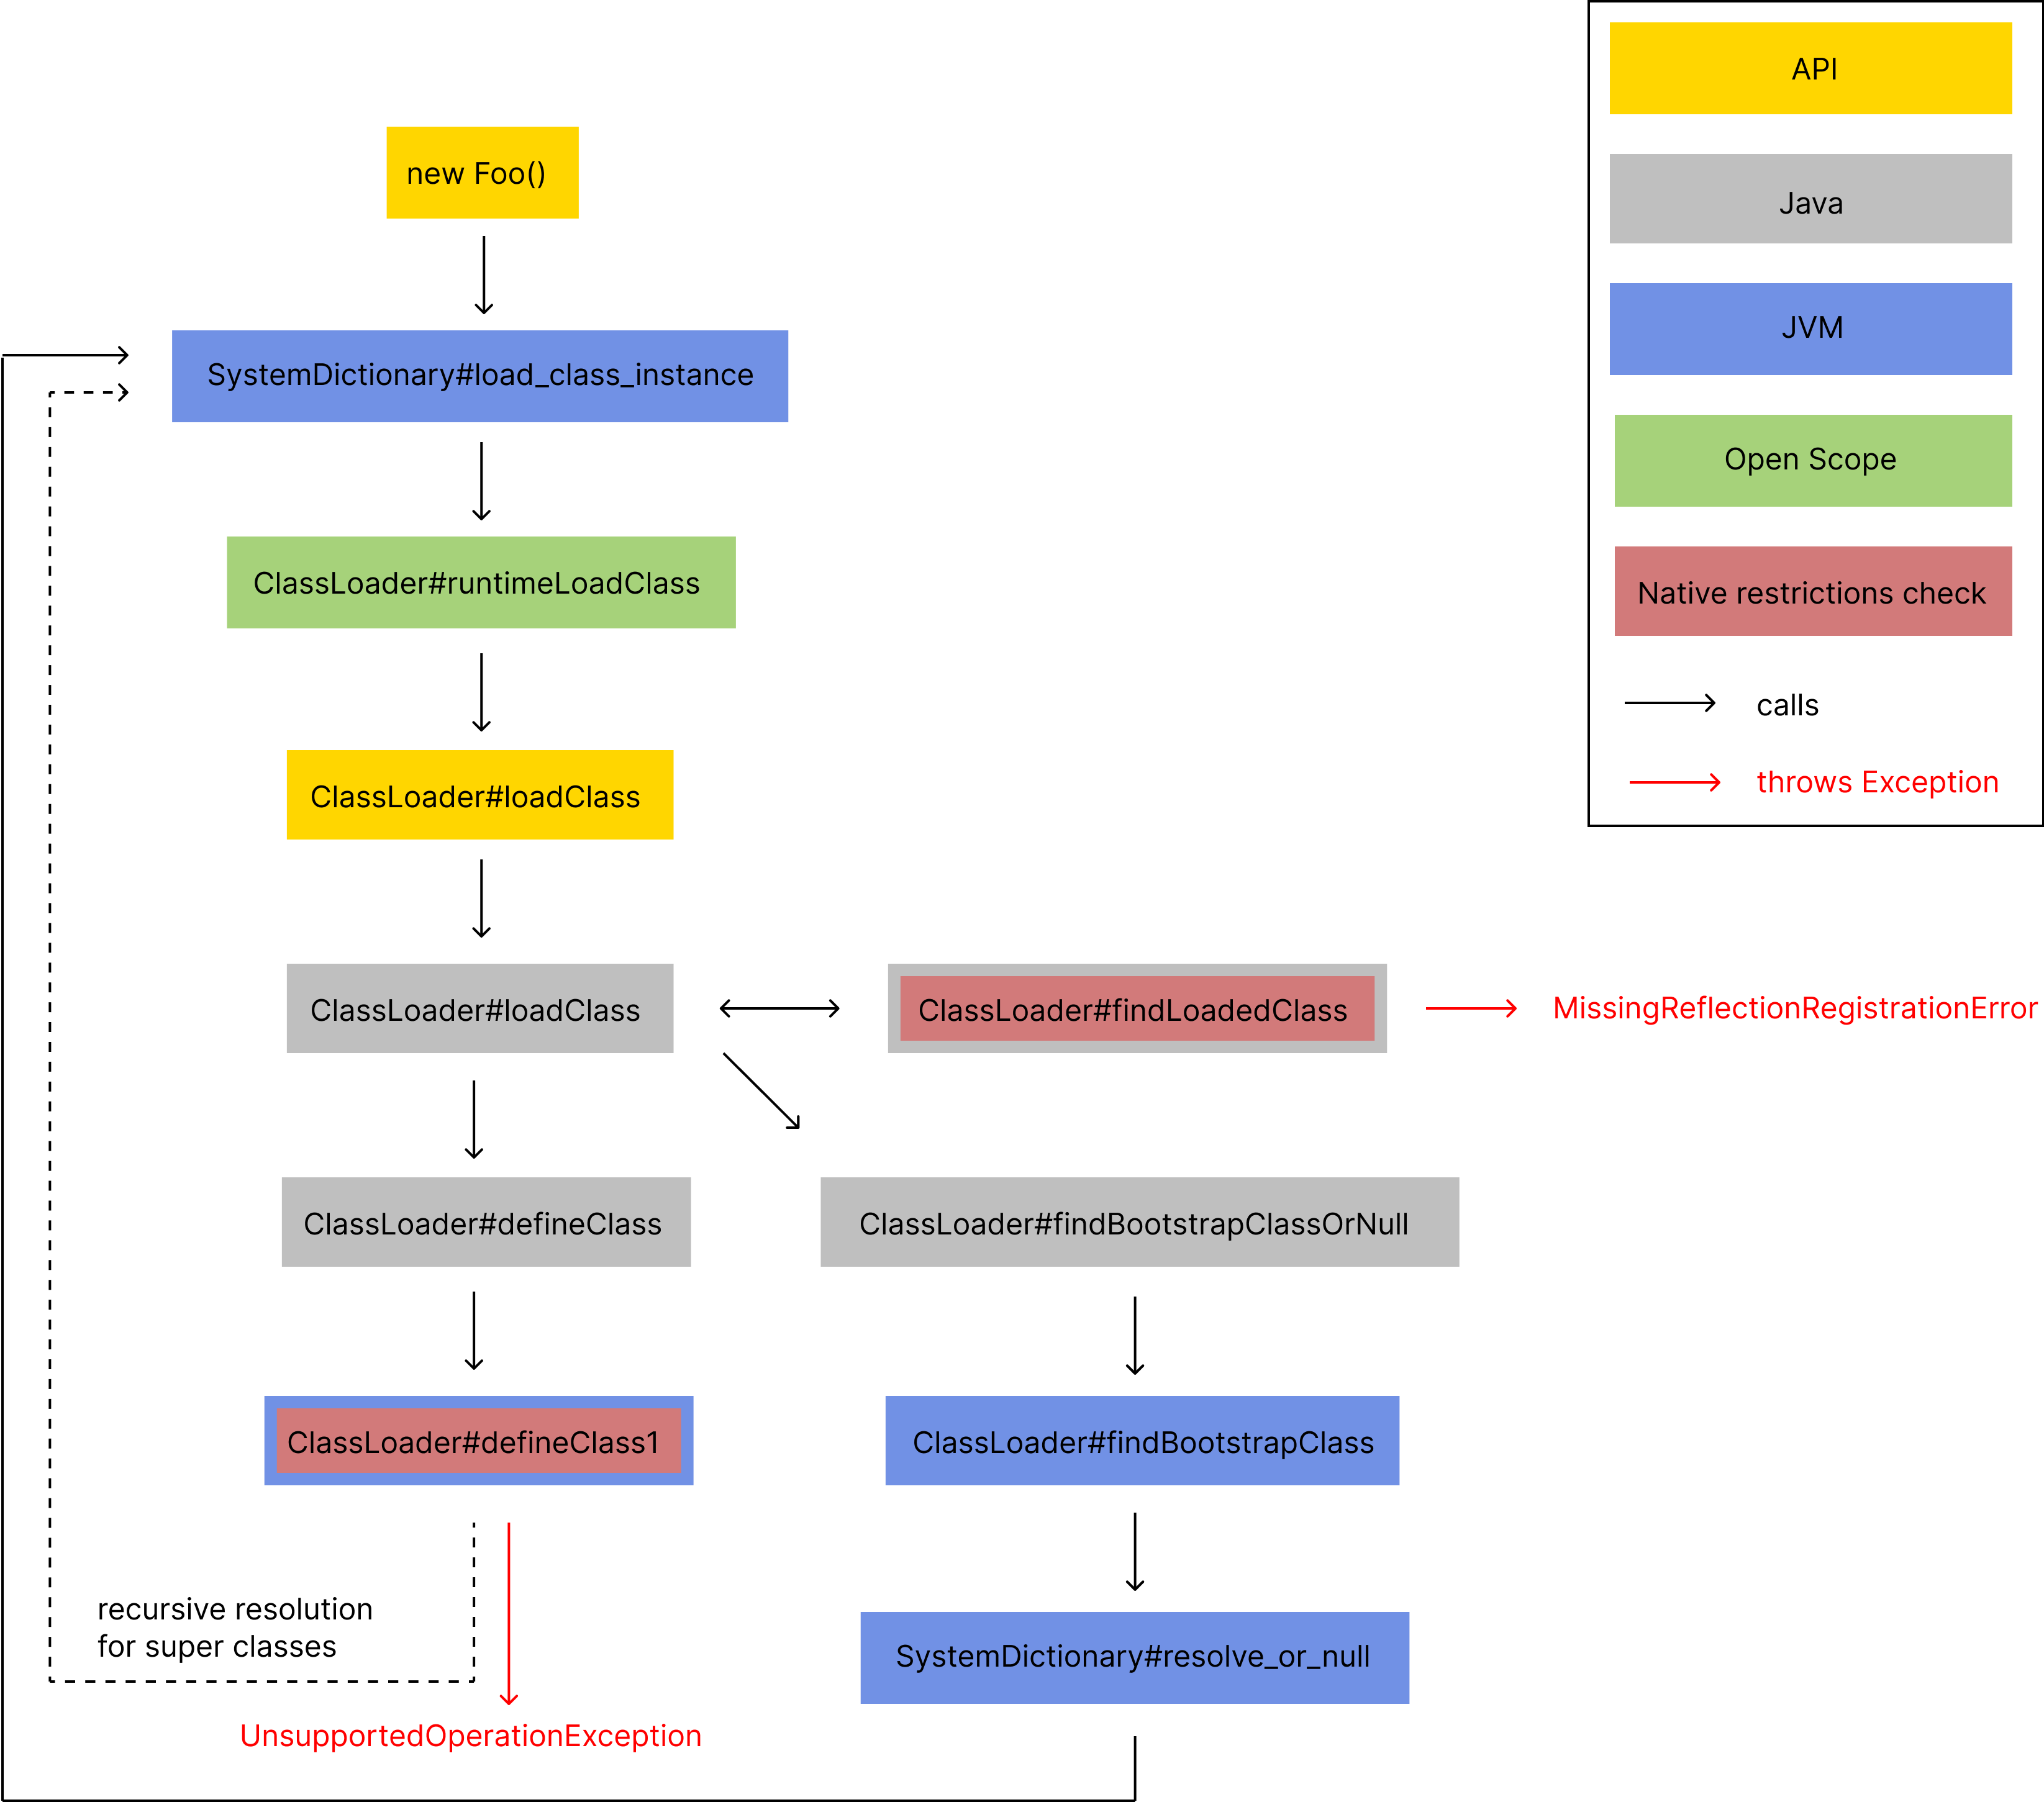
\includegraphics[scale=0.5]{resources/Group 412.png}
    \caption{Calling sequence for class loading, with the wrapper function \texttt{runtimeLoadClass} and scopes to support dynamic class loading at runtime.}
    \label{fig:load_class}
\end{figure}

The design of dynamic invocation under native restrictions required multiple iterations to keep the changes to a minimum. Figure~\ref{fig:define_class_0} shows all the entry points from which \verb|java.lang.ClassLoader#defineClass0| can be invoked to define a hidden class as part of the of the dynamic invocation process and illustrates the final state of the design. 

Under native restrictions the methods \verb|metafactory| and \verb|altMetafactory| of \verb|java.lang.invoke.LambdaMetfactory| throw an \verb|UnsupportedOperationException| to prevent the execution of arbitrary code at runtime, unless the invocation is part of the \verb|invokedynamic| instruction.
To differentiate both behaviours, we open a scope in \verb|java.lang.BootstrapMethodInvoker#invoke|. The method is invoked by the JVM in the process of linking the \verb|CallSite|, when resolving the bootstrap method. Following Native Image's semantics, the scope is opened if and only if Native Image also compiles this bootstrap method at build time. Figure~\ref{fig:define_class_0}, shows that moving the opening of the scope up or down on the stack trace would introduce an additional change because of the branching out. We also do not have the required metadata on the bootstrap method to place it in the JVM.

% Certain user calls can trigger the definition of internal Java classes at runtime, for performance reason we treat these calls differently in Java under native restrictions.
Specific user calls can trigger the definition of internal Java classes at runtime; for performance reasons, we treat these calls differently in Java under native restrictions.
Concretely, the invocation or binding of a method handle and the lookup of an executable or field can result in the resolution of a method handle such that the JVM emits instructions to define internal classes of Java at runtime. During the resolution process, the JVM can, as an optimization, compile internal classes, such as a \verb|java.lang.invoke.LambdaForm| and specialized form of \verb|BoundMethodHandle|.
In Native Image, these hidden classes are forced-interpreted, and method handles are resolved through reflection. As such, letting Java under native restrictions define these classes and defer the restrictions checks to the resolution of method handle, as seen in the next section, does not contradict the semantics of Native Image. Therefore, for performance reasons, we opt to open scopes in \verb|jdk.internal.reflect.MethodAccessGenerator#invoke|, and in the methods \verb|InvokeBytecodeGenerator#loadMethod|, \verb|MethodHandle.BindCaller#makeInjectedInvoker|, and \verb|ClassSpecializer#loadSpecies| of the \verb|java.lang.invoke| package. These changes correspond to the top part of the stack traces on the graph of Figure~\ref{fig:define_class_0}. By the same process as the \verb|LambdaMetfactory|, and because none of the paths that need to implement native restrictions checks systematically meet at a node, we can prove that moving any of the scopes up or down on the stack trace would lead to the same amount or strictly more modifications.

\begin{figure}
    \centering
    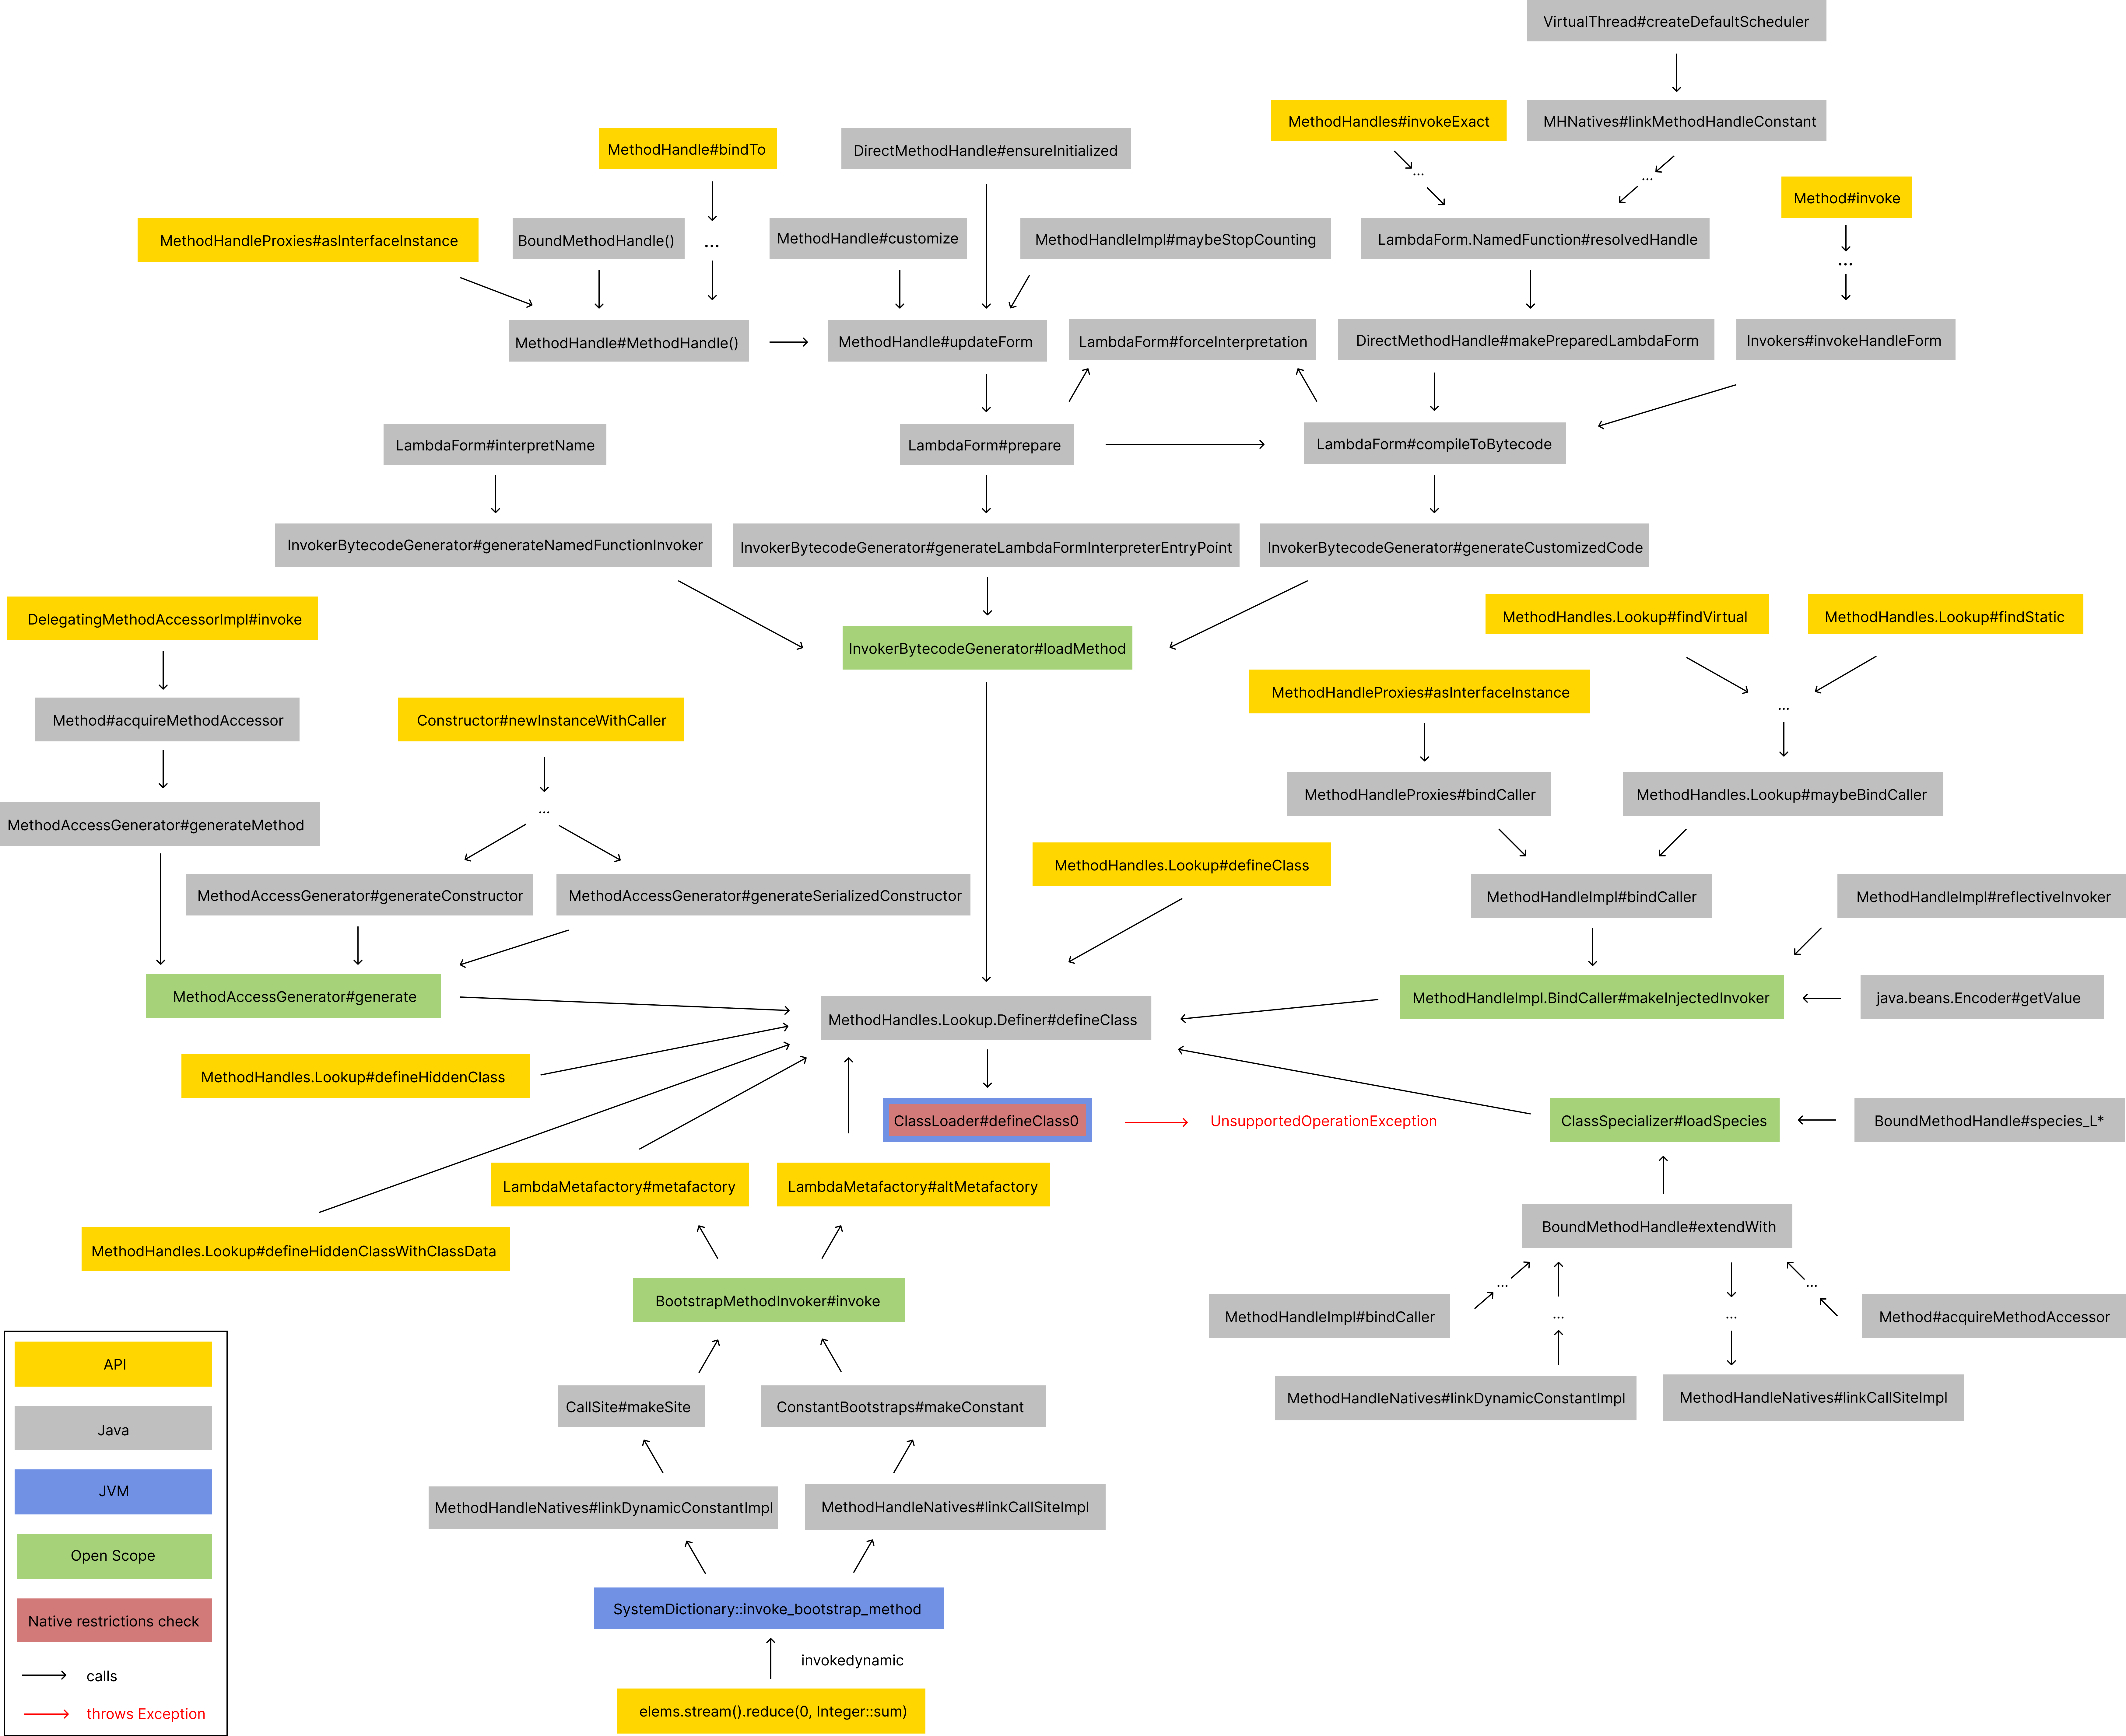
\includegraphics[angle=90,origin=c,scale=0.35]{resources/Group 413.png}
    \caption{Entry points for the method \texttt{java.lang.ClassLoader\#defineClass0}. For readability, the stack trace is not exhaustive and focuses on methods that have multiple callers.}
    \label{fig:define_class_0}
\end{figure}


Since the Java Native Interface~(JNI)~\cite{noauthor_jni_nodate} allows users to make downcalls to the JVM's implementation of the methods \verb|defineClass1|, \verb|defineClass2|, and \verb|defineClass0|, the native restriction checks must be placed in the JVM rather than in Java. We insert the checks in the JVM's method \verb|SystemDictionary::resolve_from_stream|, which is part of the common code for \verb|JVM_DefineClass| and \verb|JVM_DefineClassWithSource|. If none of the scopes are open, the call will result in an \verb|UnsupportedOperationException|. 

Through a static study of entry points and stack traces and the introduction of a few native restrictions scopes, we prove that the semantics of Java for dynamic class loading can be changed such that it simulates Native Image's.

%%%%%%%%%%%%%%%%%%%%%%%%%%%%%%%%
\subsection{Reflection}
%%%%%%%%%%%%%%%%%%%%%%%%%%%%%%%%
Modifying the reflection feature under native restrictions consists in adding native restrictions checks to all methods in the class \verb|java.lang.Class|, the package \verb|java.lang.invoke.reflect|, and \verb|jdk.internal.sun.misc.Unsafe|, that returns a reflectively-accessed element. Section~\ref{native_image_specs} describes the list of checks in more detail. 
If the element is not registered for reflection, a \verb|MissingReflectionRegistrationError| is thrown.
To check if an element is registered, we load all JSON reflection configuration files that are on the classpath or user-defined. The classes and interfaces to parse the JSON reflection configuration file and the data structure that holds the configuration are taken directly from Native Image. Changes made to that part of the code in Native Image can be easily adapted to work in Java under native restrictions.

In Java under native restrictions we modify the process of \verb|MethodHandle| resolution to match Native Image's semantics.
The resolution of a method handle can occur, from the user perspective, either as the result of the dynamic invocation of a method or as the result of a lookup.
Similarly to reflection, \verb|java.lang.MethodHandles.Lookup| provides an API to look up \verb|Executables|, \verb|Fields|, and \verb|VarHandles|, and returns a method handle to access the element. 
In Native Image, the \verb|MemberName| encapsulated in the method handle is resolved through reflection if it does not reference an intrinsic method. To simulate this behaviour in Java under native restrictions, we introduce a native restriction check in the \verb|java.lang.invoke.MemberName#resolve|. 
For intrinsic methods, we keep a hard-coded list of \verb|MemberName| that do not require reflection to be resolved. Scopes cannot be used in this case, as invoking any method to open a scope relies on these same intrinsic method handles.
Moreover, as parts of the internal code for reflection configuration use lambda expressions, we also open a scope in \verb|MethodHandles#linkMethodHandleConstant| to prevent cyclic dependencies.

During reachability analysis, Native Image can prove that internal classes accessed reflectively from the Java language to the Java language are reachable and do not need to be specified in the metadata. 
%Internally, the JVM uses reflection to access internal Classes, Executables and Fields. 
To invoke a method obtained via a lookup, for example, the JVM will reflectively access the method \verb|java.lang.invoke.MethodHandle#invokeBasic|. Because Native Image can prove from the code that these elements are reachable, these calls from the JVM to the JVM are not constrained to native restrictions. To filter out these accesses, Java under native restrictions implements an \verb|AccessAdvisor|, adapted from the \verb|AccessAdvisor| used by GraalVM's Tracing Agent. The advisor contains a list of classes and patterns (e.g., \verb|java.lang.**|), such that if the caller at the origin of the reflective access is included in that list, the native restrictions checks are ignored.

Building on top of Java under native restrictions for dynamic class loading, we add native restrictions checks to verify that every reflectively-accessed element is registered for reflection and we introduce an \verb|AccessAdvisor| to filter out calls from the JVM to the JVM that can safely be ignored.

%%%%%%%%%%%%%%%%%%%%%%%%%%%%%%%%
\section{Improving Usability}
%%%%%%%%%%%%%%%%%%%%%%%%%%%%%%%%
In this section, we will see how Java under native restrictions fits in the overall Native Image usability plan by improving the turnaround for computing reachability metadata and defining the expected behaviour of Native Image. 

%%%%%%%%%%%%%%%%%%%%%%%%%%%%%%%%
\subsection{Streamlining reachability metadata computation}
%%%%%%%%%%%%%%%%%%%%%%%%%%%%%%%%
One of the primary goals of this thesis is to streamline reachability metadata computation for users.
The first step in the computation of the metadata is the collection. To achieve this, GraalVM's Tracing Agent automatically collects the reachability metadata required for an application. The issue with the current implementation is that the JVM to which it is attached does not follow Native Image's semantics. As a result, the agent can take an entirely different path during execution than Native Image, and miss reflectively-accessed elements. Moreover, attaching an agent to the JVM significantly slows down the execution.
Our solution to this problem is to implement another Tracing Agent in Java. The Tracing Agent is another language restriction designed to follow the exact same path during an execution as Java under native restrictions. Instead of performing restriction checks, the agent logs the reflectively-accessed elements and outputs a JSON reflection configuration at the end of the execution run. 
Once the metadata are collected, the configuration can be tested on Java under native restrictions, thus avoiding the overhead of building an image. The Evaluation Section~\ref{benchmark} illustrates that this overhead is non-negligible when it comes to testing.  

We propose a new and optimized workflow for computing metadata: (1) run the agent, (2) test the JSON reflection configuration with Java under native restrictions, (3.a) if the execution did not result in an exception, build the image, (3.b) otherwise debug the application by attaching a Java debugger to Java under native restrictions if needed.

%%%%%%%%%%%%%%%%%%%%%%%%%%%%%%%%
\subsection{Defining expected behaviour}
%%%%%%%%%%%%%%%%%%%%%%%%%%%%%%%%
The Technology Compatibility Kit~(TCK) is our first approach to specifying the semantics of Native Image for dynamic class loading and reflection. The TCK is a test suite that illustrates the specifications. It gives concrete examples of the expected behaviours and provides a future-proof way of asserting that different versions of Native Image still behave according to the same semantics.
It is designed to run with both Native Image and Java under native restrictions.

Test harnesses usually rely on annotations to get the test classes and individual tests to run, but using reflection in the TCK to test reflection is not an option. JUnit's~\cite{noauthor_junit_nodate} \verb|@Test| annotation on methods, for example, can be reflectively queried to obtain the test \verb|Method| to invoke in the test harness. Instead, we rely on an annotation processor to generate on the fly all the data structure needed to run the test harness at compile time without using any reflective call (see Section~\ref{TCK} for details on the implementation).

The TCK contains positive and negative unit tests for dynamic class loading and reflection. To guarantee the correctness of the tests themselves, in particular for reflection, each test uses reflection on different dummy classes, so that the tests do not interfere with each other.
The test uses the \verb|opaque| method, as seen in Figure~\ref{fig:opaque}, to wrap arguments passed for reflection and ensure that no compiler optimization is done across the call.

\begin{figure}[ht]
    \centering
\begin{lstlisting}[language=Java]
public static <T> T opaque(T value) {
    System.out.printf("");
    return value;
}
\end{lstlisting}
    \caption{The \texttt{opaque} method does nothing but ensures that the provided argument does not get constant-folded by the compiler.}
    \label{fig:opaque}
\end{figure}

Despite - or thanks to - its simplicity, the TCK did enable us to catch bugs in Native Image. Some of the bugs, as seen in Figure~\ref{fig:new_multi_array_bug}, are easy to fix, as Native Image only returns the wrong type of exception.  
Instantiating a new array is supported in Native Image if the component type of the array is registered for reflection. However, currently, trying to instantiate a new array without registering \texttt{C} for reflection throws a fatal error \texttt{java.lang.IllegalArgumentException} that cannot be caught instead of throwing a \verb|MissingReflectionRegistrationError|. Similarly, trying to instantiate a new multi-dimension array without registering \texttt{C} for reflection throws a \texttt{com.oracle.svm.core.jdk.UnsupportedFeatureError}, even though the feature is supported and only requires the class to be registered to work.

\begin{figure}[ht]
    \centering
\begin{lstlisting}[language=Java]
class C {
}

class Main {
    public static void main(String[] args) throws Exception {
        Array.newInstance(opaque(C.class), 5);
        Array.newInstance(opaque(C.class), 5, 5);
    }
}
\end{lstlisting}
    \caption{Example of bug caught with the TCK where Native Image's behaviour deviated from the expected behaviour.}
    \label{fig:new_multi_array_bug}
\end{figure}

We found another bug with the TCK, which concerned the registration of superclasses. For a class \verb|B| that extends \verb|A|, if \verb|B| is registered for reflection but \verb|A| is not, then invoking \verb|Class#forName(opaque("A"))| still returns the class without throwing an exception, which is wrong according to Native Image's semantics. 
We also found a performance bug for a preview feature of Java 21. The \verb|java.util.FormatProcessor| uses a bootstrap method that Native Image currently interprets. Over 100'000 iterations, running the program shown in Listing ~\ref{fig:format_processor} with Native Image is 2X slower than with HotSpot. This bootstrap method can be proven safe to compile at build time, and the overhead of interpreting it at runtime could be avoided. By compiling the method, we can obtain a speedup of 3X compared to HotSpot.

\begin{figure}[ht]
    \centering
\begin{lstlisting}[language=Java]
public class Main {
    public static void main(String[] args) {
        String str = FormatProcessor.FMT."Hello there!";
    }
}
\end{lstlisting}
    \caption{The \texttt{FormatProcessor} uses the bootstrap method \texttt{java.lang.runtime.TemplateRuntime.processStringTemplate}, which can be proven safe to compile at build time. }
    \label{fig:format_processor}
\end{figure}

The TCK provides a representation of Native Image's semantics and proves that with a few unit tests and a clear semantics, we can already improve Native Image usability by detecting unexpected behaviours.
% Balance between what needs to be changed in Native Image, driving the specs with this Java mode, and using part of what is in Nativ eImage in Java mode (e.g. 
% MissingReflectionRegistrationError is still in progress in Native Image, but also using in Java).

% Building the agent after doing the defineClass -> back and forth
% SecurityManager was changed in Java moide, so had to change in NI, but other changes were made in NI so also had to propagate back the changes into the Java mode.
% etc.

%%%%%%%%%%%%%%%%%%%%%%%%%%%%%%%%
\chapter{Implementation}
%%%%%%%%%%%%%%%%%%%%%%%%%%%%%%%%
% The implementation covers some of the implementation details of your project.
% This is not intended to be a low level description of every line of code that
% you wrote but covers the implementation aspects of the projects.
% Please provide as stable as possible links to the implementation source code.

This section discusses implementation details of the native restrictions, the scopes and checks, and the TCK.

%%%%%%%%%%%%%%%%%%%%%%%%%%%%%%%%
\section{LanguageRestrictionManager}
%%%%%%%%%%%%%%%%%%%%%%%%%%%%%%%%
The \verb|LanguageRestrictionManager| is the main entry point to the language restrictions. It provides a singleton instance of the abstract class \verb|LanguageRestriction|, which is the superclass of: 
\begin{itemize}
    \item \texttt{NativeLanguageRestriction} which models Native Image semantics
    \item \texttt{NoLanguageRestriction} which  models Java semantics
    \item \texttt{NativetraceLanguageRestriction} for the Java Tracing Agent that we implemented
\end{itemize}
The type of \verb|LanguageRestriction| is selected by setting the System property \verb|language.restriction| to either \verb|'native'|, \verb|'none'| or \verb|'native-trace'|. 

The \verb|LanguageRestrictionManager| is the interface for every native restrictions checks, and is used to hide away the scope abstraction when possible.
The language restriction is initialized during the last phase of the VM initialization and loads the reflection configuration.
% object into an instance of \verb|TypeConfiguration|, 
%%%%%%%%%%%%%%%%%%%%%%%%%%%%%%%%
\section{Native Restrictions Scopes}
%%%%%%%%%%%%%%%%%%%%%%%%%%%%%%%%
We implemented native restrictions scopes with thread local counters. Using thread locals prevents the opening of a scope on one thread from interfering with another thread's scopes.
Concretely, each time a scope is opened, the counter is incremented, and each time a scope is closed, the counter is decremented. The counter also accounts for recursive calls: the scope is either open or closed until the base case of the recursion returns.
To avoid memory leaks, the thread local is instantiated in a \verb|try-with-resource| block statement (see Figure~\ref{fig:bind_caller_twr}) and implements the \verb|AutoCloseable| interface, which calls the method \verb|close| to release resources on return or when an exception occurs.

\begin{figure}[ht]
    \centering
\begin{lstlisting}[language=Java]
static MethodHandle bindCaller(MethodHandle mh, Class<?> hostClass) {
    try (NativeRestrictions unused = NativeRestrictions.openScope()) {
        return BindCaller.bindCaller(mh, hostClass);
    }
}
\end{lstlisting}
    \caption{Explicit try-with resource block statement to open a scope in Java under native restrictions.}
    \label{fig:bind_caller_twr}
\end{figure}

As seen in Figures~\ref{fig:bind_caller_lambda} and~\ref{fig:bind_caller_lrm}, to minimize the changes made to Java, the \verb|try-with-resource| block statement is hidden in the \verb|LanguageRestrictionManager| and the region of code that was in the block in Figure~\ref{fig:bind_caller_twr} is passed as a lambda expression and invoked in the \verb|LanguageRestrictionManager|. Hiding the scope opening in a lambda is only possible for a region of code that is not on the path of an \verb|invokedynamic| instruction, as this would create a cyclic dependency. 

\begin{figure}[ht]
    \centering
\begin{lstlisting}[language=Java]
static MethodHandle bindCaller(MethodHandle mh, Class<?> hostClass) {
    return LanguageRestrictionManager.bindCallerCheck(() -> 
        BindCaller.bindCaller(mh, hostClass));
}
\end{lstlisting}
    \caption{Lambda expressions are used to hide implementation details in the \texttt{LanguageRestrictionManager} and minimize changes made to the JDK.}
    \label{fig:bind_caller_lambda}
\end{figure}

\begin{figure}[ht]
    \centering
\begin{lstlisting}[language=Java]
public static MethodHandle bindCallerCheck(Supplier<MethodHandle> s) {
    try (NativeRestrictions unused = NativeRestrictions.openScope()) {
        return s.get();
    }
}
\end{lstlisting}
    \caption{Implementation of the native restrictions checks in the \texttt{LanguageRestrictionManager} when the supplier \texttt{s} is passed as a lambda expression from the JDK.}
    \label{fig:bind_caller_lrm}
\end{figure}

%%%%%%%%%%%%%%%%%%%%%%%%%%%%%%%%
\section{Technology Compatibility Kit}\label{TCK}
%%%%%%%%%%%%%%%%%%%%%%%%%%%%%%%%
The TCK is a test suite for Native Image and Java under native restrictions that tests Java's dynamic features and reflection. 
%As the test harness cannot rely on reflection, we use an annotation processor to generate all the data structures needed to invoke the tests. 
It is Gradle~\cite{noauthor_gradle_2024} project composed of 4 sub-projects: 
\begin{itemize}
    \item the \verb|annotation-processor| contains all the logic for the annotation processor and the generation of scripts to run the TCK
    \item the \verb|tck| contains the tests classes
    \item the \verb|tck-harness| contains the test harness to run the test and asserts the results
    \item the \verb|tck-utils| contains common utility classes
\end{itemize}
The separation of the features into sub-projects simplify the compilation chains, as the first three sub-projects depend on the \verb|tck-utils|, the \verb|tck| depends on the \verb|annotation-processor|, and the \verb|tck-harness| depends on the \verb|tck|.

The TCK aims to assert that Native Image and Java under native restrictions follow the correct semantics. Therefore, it must also be able to run tests both with and without reachability metadata. Since, by default, all tests in a test class share the same metadata and are built into a single image for Native Image, a second requirement is that a test should be able to run in isolation and have its own separate image and metadata. 
Figure~\ref{fig:tck_for_name} is an example of a test that the TCK can run. Each test in the suite is annotated with the \verb|@Test| annotation. The annotation contains fields for the reflection metadata, for the expected exception when the test runs without the metadata, and an optional field \verb|sinceVersion|, if a previous version of Native Image did not behave as expected. The \verb|@NativeImageTCKDeviation| means that the current version of Native Image does not return the expected behaviour. Finally, \verb|@RunTestInIsolation| can be used to run the test in an isolated image. 

\begin{figure}[ht]
    \centering
\begin{lstlisting}[language=Java]
@Test(
    reflectionMetadata =
            """
            [{
                "name": "ForNameTestClass"
            }]
            """,
    expectedNoRegistrationException = MISSING_REFLECTION_REGISTRATION_ERROR
)
@RunInIsolation
@NativeImageTCKDeviation(ticketNumber = "GR-123456")
public static void forName() throws Exception {
    Class<?> result = Class.forName(opaque("ForNameTestClass"));
    assertEquals(opaque(ForNameTestClass.class), result);
}
\end{lstlisting}
    \caption{Example of a test that expects a \texttt{ForNameTestClass.class} to be returned when the class is registered and a \texttt{MissingReflectionRegistrationError} to be thrown otherwise. It runs in its own \texttt{native-image} and the issue \texttt{GR-123456} has been filed because Native Image does not currently behave as expected.}
    \label{fig:tck_for_name}
\end{figure}

To implement these features, the annotation processor does most of the heavy lifting. The annotation parsing phase is made of three steps:
\begin{enumerate}
    \item It maps each test class to a list of \verb|TestData| Records 
    \item It parses the \verb|reflectionMetadata| field of each test and generates the associated JSON reflection configuration in a \verb|reflect-config.json| files
    \item It generates bash scripts for Native Image and Java with the command to run the test harness with and without metadata for each test class and isolated test
\end{enumerate}
The \verb|TestData| contains, for each test, the expected results when running without registration, an optional \verb|sinceVersion|, a boolean for if it should run in isolation and if Native Image's behaviour deviates, and a \verb|Callable|, such that the test harness can invoke the method without relying on reflection.  
A \verb|TestRunnerMap.java| file is automatically generated during the annotation parsing, and contains the map described in 1., with its entry statically initialized. 

To run the tests in the TCK, the test harness instantiates an instance of \verb|TestRunnerMap| at runtime, iterates through the entries, invokes the \verb|Callable| in the \verb|TestData|, and asserts that the returned result is correct.

%%%%%%%%%%%%%%%%%%%%%%%%%%%%%%%%
% \section{Dynamic Class Loading}
%%%%%%%%%%%%%%%%%%%%%%%%%%%%%%%%
% Native Image does not allow for runtime definition of classes that were not preloaded beforehand.
% To simulate this behaviour, we introduce the wrapper method java.lang.ClassLoader#runtimeLoadClass. The only entry point for this private method is the interpreter. If not preloaded, then a class may be defined at runtime only if resolving the class or interface was required by one of the following instructions:
% anewarray, checkcast, getfield, getstatic, instanceof, invokedynamic, invokeinterface, invokespecial,
% invokestatic, invokevirtual, ldc, ldc\_w, multianewarray, new, putfield, and putstatic.
% The wrapper then dispatches the call to the method loadClass to the delegate class loader, as intended when running without restrictions.
% Runtime calls to the public method java.lang.ClassLoader#loadClass methods first checks if the class was preloaded (i.e. checking the inclusion of the class in the reflection metadata is sufficient to simulate Native Image behaviour in this Java mode), before allowing it to be defined.

%%%%%%%%%%%%%%%%%%%%%%%%%%%%%%%%
\chapter{The Native Image Reflection Semantics}\label{native_image_specs}
%%%%%%%%%%%%%%%%%%%%%%%%%%%%%%%%


%% TODO add snippets of code to show how it differes from normal Java

% ## Unimplemented Features
% #### java.lang.SecurityManager
% The `java.lang.SecurityManager` behaves in the following ways:
% * `java.lang.System#getSecurityManager()` always returns `null`
% * `java.lang.System#setSecurityManager(SecurityManager sm)` returns without exception if `sm` is null. 
% It throws a `SecurityException` if the system property `java.security.manager` is not set to `disallow`, and an 
% `UnsupportedOperationException` otherwise.


%%%%%%%%%%%%%%%%%%%%%%%%%%%%%%%%
\chapter{Evaluation}
%%%%%%%%%%%%%%%%%%%%%%%%%%%%%%%%
% In the evaluation you convince the reader that your design works as intended.
% Describe the evaluation setup, the designed experiments, and how the
% experiments showcase the individual points you want to prove.
In this section we show that the design of Java under native restrictions is correct according to Native Image's semantics and that it allows for visible improvements when it comes to testing the reachability metadata configuration.

%%%%%%%%%%%%%%%%%%%%%%%%%%%%%%%%
\section{Correctness of Java under native restrictions}
%%%%%%%%%%%%%%%%%%%%%%%%%%%%%%%%
To verify that Java under native restrictions is indeed correct with regard to the semantics of Native Image, we run the TCK with and without the reachability metadata and assert that our implementation does throw an exception in the correct place when the metadata is missing and returns the expected results otherwise. This evaluation step trivially succeeded, as the development of Java under native restrictions was partly test-driven by the TCK.

The other way of asserting the correctness of our implementation is with the JCK. The JCK is a proprietary test suite from Oracle that is used used to assert that a Java implementation complies with the Java Language Specification. A CI job is available on the enterprise repository to run the JCK for Native Image. The CI job has three stages:
\begin{enumerate}
    \item The JCK is run with GraalVM's Tracing Agent to collect all the metadata
    \item An images is built for each test with the collected metadata
    \item The images are executed
\end{enumerate}
For Java under native restrictions we adapted the stages such that the first one used our implementation of the Tracing Agent, the build stage is altogether skipped, and the image run stage is replaced with a Java under native restrictions run stage.

The evaluation criteria we observe when running the JCK with Java under native restrictions is whether our implementation is at least as compliant as Native Image is. Currently, Native Image does not pass all the JCK tests. Some tests fail because they are transients or attempt to test unsupported or not yet implemented features. Other tests fail because they contradict Native Image's Semantics. For example, tests that dynamically load a class at runtime that is not on the classpath should fail in both Native Image and Java under native restrictions. 

For the JCK we obtained the following result: Java under native restrictions passes all the tests of the JCK that Native Image does and also fails where Native Image fails, except for 17 specific tests out of the 115'464. Native Image has a special class loader, used for features like the JMX framework, that enables dynamic class loading of classes from another module. Since Java under native restrictions does not implement this feature, one limitation is that we do not support connection to a remote RMI connector (i.e., instantiating a \verb|javax.management.remote.rmi.RMIConnector| throws an \verb|UnsupportedOperationException|). 
Moreover, some tests are transients when run with Java under native restrictions but not in Native Image. The reason could be that, in these tests, the agent follows a different path when operating in a concurrent setting and cannot record all the reflectively-accessed elements on every path. 

A current limitation of Java under native restrictions concerns dynamic proxies and resource bundles. These are two dynamic features of Java that can be used to access and load new elements at runtime. In Native Image these two features are treated differently than reflectively-accessed elements and have their own separate JSON reflection configuration files in the reachability metadata. Java under native restrictions does not currently implement native restrictions checks for dynamic proxies and resources. Therefore, it is still possible to dynamically load these elements at runtime, without specifying them in the metadata. 

%%%%%%%%%%%%%%%%%%%%%%%%%%%%%%%%
\section{Benchmarks for Java under native restrictions and Native Image}\label{benchmark}
%%%%%%%%%%%%%%%%%%%%%%%%%%%%%%%%
In this section, we show that Java under native restrictions can be successfully used to streamline the computation of reachability metadata. The benchmarks were conducted on a 20 cores 13th Gen Intel(R) Core(TM) i7-1370P machine with 32GB of RAM. The two sets of experiments are run on the same Java program shown in Figure~\ref{fig:benchmark}. 

\begin{figure}[ht]
    \centering
\begin{lstlisting}[language=Java]
class C {
    public C() {}
    public String greet() {
        return "Hello there!";
    }
}

public class Main {
    public static <T> T opaque(T value) {
        System.out.print("");
        return value;
    }
    public static void main(String[] args) throws Throwable {
        ClassLoader cl = new ClassLoader() {};
        Class<?> clazz = cl.loadClass(opaque("C"));
        Method greet = clazz.getMethod("greet");
        Constructor<?> ctor = clazz.getConstructor();
    }
}
\end{lstlisting}
    \caption{Test scenario that performs three reflective access for three different elements: one to load the class, another to get the Method \texttt{greet}, and the last one to get the Constructor.}
    \label{fig:benchmark}
\end{figure}

In the first benchmark, we compare the run time of Java under native restrictions, Java under native restrictions with the new Tracing Agent, Oracle OpenJDK 21, and Oracle OpenJDK21 with GraalVM's Tracing Agent attached, when all reflectively-accessed elements are correctly registered.
We take the average of 10 runs, where each run executes 10'000 times the main method.
Figure~\ref{tab:benchmark_1} shows that Java under native restrictions and Java under native restrictions with the Tracing Agent are naturally slower than Oracle OpenJDK, due to the native restrictions checks that both Java modes need to perform at runtime to simulate Native Image behaviour or to collect the metadata. 
The takeaway of this experiment is that computing the reachability metadata with the new Tracing Agent is 5.5X faster than GraalVM's.

\begin{table}[ht]
\centering
\begin{tabular}{@{}lr@{}}
\toprule
                               & \multicolumn{1}{l}{Execution time (ns)} \\ \midrule
Java under native restrictions & 28343                                   \\
Java's Tracing Agent           & 11409                                   \\
Oracle OpenJDK 21              & 739                                     \\ 
GraalVM's Tracing Agent        & 63481                                   \\ \bottomrule
% Native Image                   & 305                                     \\ \bottomrule
\end{tabular}
\caption{Comparison of the execution time between 2 different Java implementations: Java under native restrictions and Oracle OpenJDK. Each JDK is also run with and without its implementation of the Tracing Agent.}
\label{tab:benchmark_1}
\end{table}

The metric we are interested in for the second experiment is the time it takes for Native Image and Java under native restrictions to crash when the reflection metadata is incomplete.
We start to time the experiment with the \verb|time| bash command once \verb|javac| has finished compiling the program into class files. 
The results for each configuration are obtained by averaging 4 runs and discarding outliers (e.g., if a run is 2X slower than previous runs, it is considered an outlier).
For Native Image we measure the time between the start of the image build process and the end of the execution of the image. Although, with such a small program, the execution time of the image is negligible, and the \verb|time| command returns 0.00s. For Java we measure the time of execution.

Let us assume we have a new programmer who has never used the reflection API in Native Image, did not read any of the documentation, and attempts to run the program in Figure~\ref{fig:benchmark}. Each time they get a \verb|MissingReflectionRegistrationError|~(MRRE), they follow the instructions in the error message and incrementally update the reachability metadata.
This approach gives an estimation of how much time it would take for them to obtain the correct metadata in Native Image versus how long it would have taken if they had used Java under native restrictions. 
In Table~\ref{tab:benchmark}, we can see that building an image for this program and waiting for it to crash at runtime takes around 3 minutes, while on Java, it takes half a second. Computing the correct metadata for this program takes 666X more time on Native Image than on Java.
This number proves that porting Java to native restrictions helps improve the turnaround for the computation of reachability metadata.

\begin{table}[ht]
\centering
\begin{tabular}{@{}lrr@{}}
\toprule
Time to MRRE (s) & \multicolumn{1}{l}{Native Image} & \multicolumn{1}{l}{Java under native restrictions} \\ \midrule
ClassLoader\#loadClass          & 192.18 & 0.23 \\
Class\#getMethod                & 231.59 & 0.28 \\
Class\#getConstructor           & 201.24 & 0.30 \\ \midrule
Total                           & 625.01 & 0.81 \\ \bottomrule
\end{tabular}
\caption{Each row of the table gives the time it takes to trigger the \texttt{MissingReflectionRegistrationError} in Native Image and Java. The first row gives the result when no metadata is registered, the second row when only the class \texttt{C} is registered, and the last row when \texttt{C} and the method \texttt{greet} are registered for reflection. The experiment shows that it takes 666x more time on Native Image than Java under native restrictions to compute the correct metadata.}
\label{tab:benchmark}
\end{table}
         % split if needed 
\chapter{Related Work}

%The related work section covers closely related work. Here you can highlight
%the related work \cite{DBLP:conf/fmcad/KuncakH21, DBLP:conf/pldi/GveroKKP13}, how it solved a problem, and why it solved a different
%problem \cite{DBLP:conf/nsdi/YabandehKKK09}. Do not repeat at length the content of related work, but rather focus
%on how it compares the present work: by enabling it, by exploring a slightly different approach \cite{DBLP:conf/cav/PiskacK08}, or by being subsumed by the current work.
%Do not play down the importance of related work. Say what is different and how
%you overcome some of the weaknesses of related work by discussing the 
%trade-offs. Stay positive and factual: do not use subjective assessment, but point out real differences.
%This section is usually 3-5 pages.
%Please use bibtex to enter publications. To find a reference, use "DBLP PaperTitle" in a search engine and then use the bib file provided by bibtex.
%Feel free to use wikipedia to find related references, but do not cite wikipedia pages themselves. Consult those pages and your advisors to find the original sources and suggestions for background material.
%%%%%%%%%%%%%%%%%%%%%%%%%%%%%%%%%%%%%%%%%%%%%%%%%%%%%%%%%%%%%%%%%%%%%%%%%%%%%%%%%%%%%%%%%%%%%%%%%%%

%%%%%%%%%%%%%%%%%%%%%%%%%
\section{Combining dynamic and static compilers}
%%%%%%%%%%%%%%%%%%%%%%%%%
Quicksilver~\cite{serrano_quicksilver_2000} is a quasi-static compiler for Java, that relies on both static and dynamic compilation. 
When a Java class is compiled, a quasi-static image~(QSI) is created. At runtime, the image is adapted such that the JVM may reuse it. If the QSI for the class does not exist, the compiler falls back to dynamic compilation to load the class. 
By first starting in a closed-world assumption and expanding to a dynamic environment when needed, this approach tackles our problem from the other direction.
Moreover, "stitching", the process used to adapt the images at runtime is quite complex. In contrast, one of the requirement for Java under native restrictions is to introduce a minimal set of changes to Java.

Another project that attempts to bridge the gap between static and dynamic compilation is Microsoft .NET Common Language Runtime~\cite{noauthor_common_2023}, an implementation of the Common Language Infrastructure~(CLI)~\cite{noauthor_common_2012}. 
Similarly to Native Image, NGen~\cite{noauthor_clr_2019} pre-compiles executables into native binaries, and resolves all dependencies at build time.
Metadata for executables are emitted by the compilers. At runtime, the metadata is checked to dynamically load classes, resolve method invocation, etc., and if needed .NET can fall back to JIT compilation.

%%%%%%%%%%%%%%%%%%%%%%%%%
\section{Reflection}
%%%%%%%%%%%%%%%%%%%%%%%%%
Reflection is an integral part of the design of Smalltalk-80~\cite{goldberg_smalltalk-80_1983}. In Smalltalk-80 everything is an object. Classes, metaclasses, and methods are all objects. Since the objects contain all the necessary metadata for reflection, the objects can be directly queried, such that instances of classes and classes themselves can be accessed and modified at runtime. 

Swift's proposal for opt-in reflection metadata~\cite{noauthor_pitch_2022} is a way to mitigate the problem that can arise because of the lack of transparency of the Reflection API, and the inclusion of unconsumed metadata in binaries. In Swift, reflection can be turned off on a module basis, which can lead to inconsistent behaviours at runtime if another module's implementation depended on reflection. Moreover, reflective calls cannot be statically analysed, and binaries can end up being polluted with unused metadata as a result. Instead of parsing a JSON configuration, Swift introduce a marker protocol called \verb|Reflectable|. This marker is checked by the compiler, so warning can be output when a module depends on the metadata, and metadata is emitted only when it is also consumed. The protocol also has the advantage of making reflection more transparent to API developers.

Like Native Image and the Java mode, Jax~\cite{tip_practical_1999} relies on a configuration file to specify which element will be reflectively accessed at runtime. They also offer an instrumented application to trace and output the metadata.

Scala Native~\cite{noauthor_scala_nodate} is an AOT compiler and a lightweight runtime for Scala that uses annotation to support reflection. Modules and classes marked with the \verb|@EnableReflectiveInstantation| can be reflectively queried at runtime by other libraries and frameworks.
This approach is similar to what we plan to implement, as this would offer the advantage of being statically analysable and more transparent for users.

%%%%%%%%%%%%%%%%%%%%%%%%%
\section{Porting programming languages}
%%%%%%%%%%%%%%%%%%%%%%%%%
`C (Tick C)~\cite{engler_c_1996} is an example of porting a static language, namely ANSI C, to a dynamic language. This allows dynamic code generation for better code optimization, but also a new kind of application like JIT compilers for C. Poletto, Hsieh, Engler and Kasshoek's tcc~\cite{poletto_c_1999} is an implementation of such a compiler. It consists of two backend, a static and a dynamic.
The former compiles the usual C or non dynamic part expressions, while the latter generates dynamic code that the static backend will then compile.

JavaScript strict mode as defined in the ECMAScript® 2024 Language Specification~\cite{noauthor_ecmascript_nodate}, is implemented along side the usual "sloppy mode", and applies another set of semantics to the language. The changes impose stricter variable naming and declaration, stricter expression scope, prohibits hoisting, and throws exception instead of silent failing. Similarly to the Java mode, Google's V8 JavaScript VM implementation~\cite{noauthor_v8_nodate}, relies on a flag system, and a "use\_strict" annotation on methods and blocks of code, to apply checks where the behaviour is expected to diverge from the sloppy mode. The main difference with our approach is that this set of semantics does not deal with dynamic features like class loading, as such no differentiation need to be made between runtime and compile time behaviour. 
%%%%%%%%%%%%%%%%%%%%
\chapter{Conclusion}
%%%%%%%%%%%%%%%%%%%%
% In the conclusion, you repeat the main result and finalize the discussion of
% your project. Mention the core results and why as well as how your system
% advances the status quo.
% 
% You may optionally include a subsection on future work, but aim to end with a concluding sentence on why the current results may have set the stage for the future.

In this thesis, we presented a solution to port Java to native restrictions and streamline the computation of reachability metadata. 
Java under native restrictions provides a way to quickly test a metadata configuration by avoiding the overhead of building an image.
By introducing native restrictions checks and scopes in Java, we showed that it was possible to modify the semantics of the language to match Native Image's while keeping the set of changes to Java itself to a minimum.

Java under native restrictions enabled us to validate and drive Native Image's semantics for dynamic class loading and reflection. These semantics are implemented both in written specifications and in the form of a TCK. Moreover, the TCK offers a future-proof mean to assert that future versions of Native Image still behave according to the same semantics. 

Finally, to address the issues of reachability metadata collection with GraalVM's Tracing Agent, we implemented another Tracing Agent in Java. This agent is, in all essence, another language restrictions that records all reflectively-accessed elements instead of enforcing native restrictions checks. The advantage of this approach is that, unlike GraalVM's agent, the Java agent follows the same semantics as Native Image. Therefore, no element is missing from the reachability metadata as a result of the JVM taking a different path during an execution run. 

% \todo{future work?} Dynamic class loading and reflection are not the only features of Java that needs reachability metadata \todo{dynamic proxies, resource bundles}
% resource bundles contains local specific resources, 
%%%%%%%%%%%%%%%%%%%%%%%%%%%%%%%%
% \chapter{Future Work}
%%%%%%%%%%%%%%%%%%%%%%%%%%%%%%%% 
% partial bytecode evaluator
% annotaitons
% build time initialization

\cleardoublepage
\phantomsection
\addcontentsline{toc}{chapter}{Bibliography}
\printbibliography

\appendix % optional appendix
\chapter{Proof of Minimal change}\label{minimal_change}

\begin{figure}
    \centering
    \includegraphics[angle=90,origin=c,scale=0.22]{resources/Group 397.png}
    \caption{Caption}
    \label{fig:define_class_0}
\end{figure}
 % split into files if needed

\end{document}